% !TeX root = ../main-paper.tex
\section{Results}

\subsection{Experiment 1: NER sensibility to the number of training samples}

Qualitative results
\textbf{TODO random samples of results + selection of failure cases}


Quantitative results: table + graph ideally (with training set size info)

\begin{table}[!h]
\caption{Experimental results of the NER models performances when trained on varying numbers of examples.}
\centering
\begin{tabular}[t]{lrcccccccc}
 & Trainset size & 49 & 99 & 199 & 398 & 796 & 1593 & 3186 & 6373\\
 & \% & 0.8 & 1.5 & 3.1 & 6.2 & 12.5 & 25 & 50 & 100\\
\midrule[1pt]\bottomrule
\multirow{3}{*}{\rotatebox{90}{F1}} & SpaCy NER & 87.0 & 89.0 & 90.3 & 91.9 & 92.1 & 92.8 & 93.2 & 93.6\\
& CamemBERT & 89.4 & 90.3 & 92.7 & 93.4 & 94.3 & 95.3 & 94.7 & 95.5\\
& CamemBERT.pretrained & 90.0 & 91.4 & 92.9 & 93.4 & 94.2 & 94.5 & 94.8 & 95.4\\
\cmidrule{1-10}
\multirow{3}{*}{\rotatebox{90}{Precision}} & SpaCy NER & 85.6 & 87.7 & 90.0 & 92.0 & 92.4 & 92.8 & 93.1 & 93.8\\
& CamemBERT & 87.3 & 88.1 & 91.4 & 93.0 & 93.4 & 95.4 & 93.8 & 95.8\\
& CamemBERT.pretrained & 87.9 & 89.8 & 91.6 & 92.7 & 93.4 & 94.0 & 94.1 & 95.4\\
\cmidrule{1-10}
\multirow{3}{*}{\rotatebox{90}{Recall}} & SpaCy NER & 88.6 & 90.4 & 90.7 & 91.7 & 91.9 & 92.8 & 93.3 & 93.3\\
& CamemBERT & 91.8 & 92.7 & 94.1 & 93.9 & 95.2 & 95.1 & 95.6 & 95.1\\
& CamemBERT.pretrained & 92.2 & 93.0 & 94.3 & 94.2 & 95.0 & 95.1 & 95.5 & 95.4\\
\end{tabular}
\end{table}

\begin{figure}[htb!]
	   \center{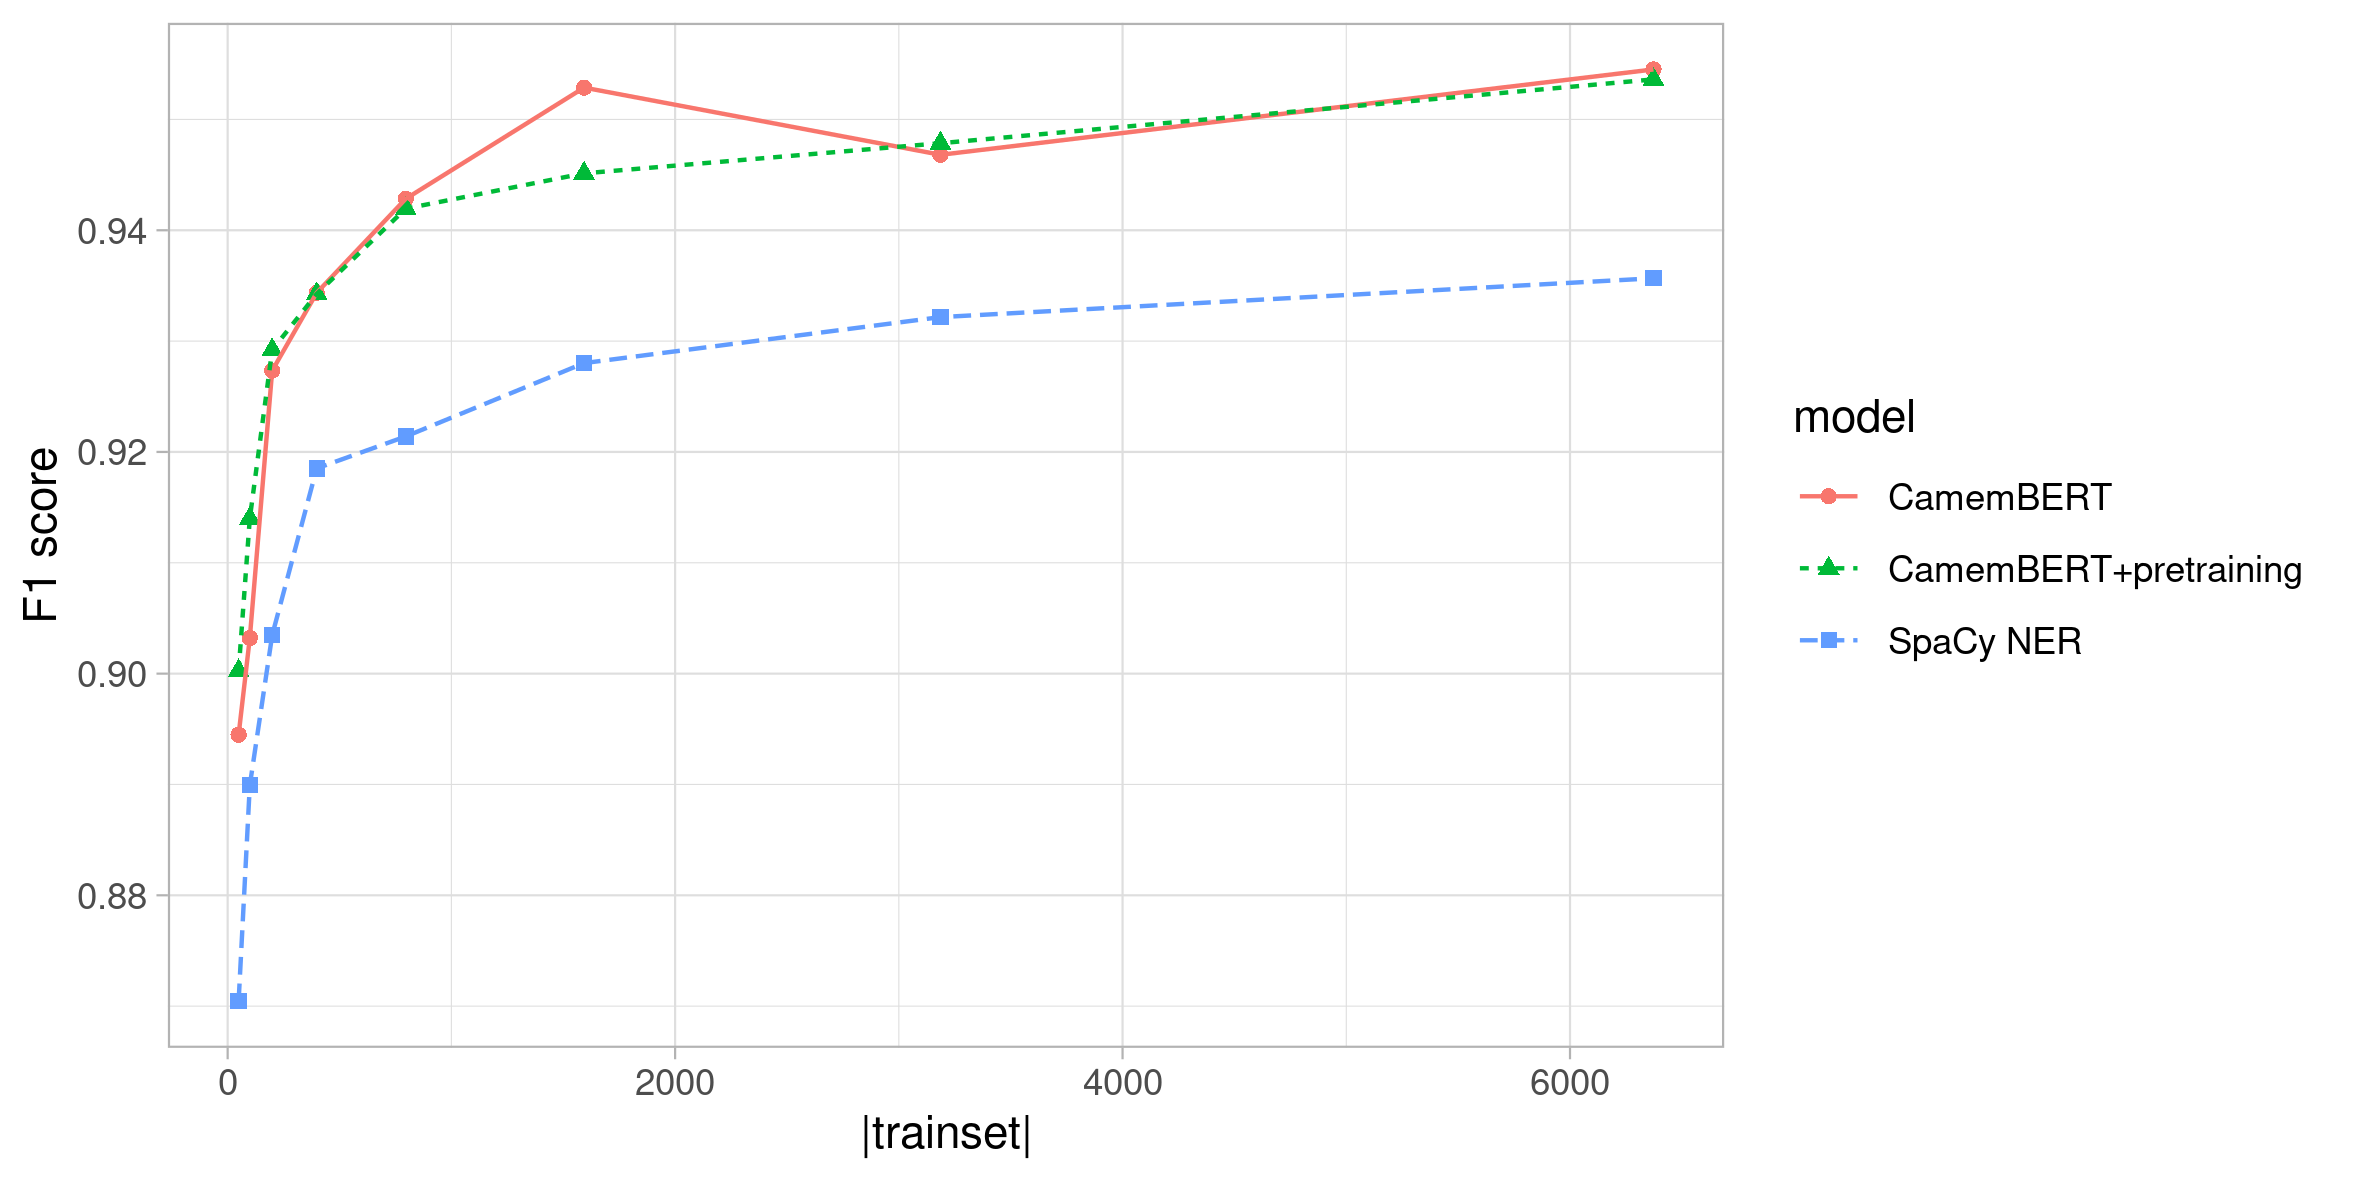
\includegraphics[width=\textwidth]
	       {../material/experiment_1/f1_vs_trainsize.png}}
	  \vspace{3in}
	  \caption{\label{fig:f1-vs-trainsize} Models F1 score on unseen data vs trainset size}
\end{figure}
	                                        


\subsection{Experiment 2: NER in the presence of noisy OCR texts}

Qualitative results
\textbf{TODO random samples of results + selection of failure cases}

Quantitative results: table + graph ideally (with OCR noise, same format as previous)

Table : NER NN models VS train on {noisy, clean} datasets VS evaluate on {noisy, clean} datasets


\begin{table}[h!]
\caption{Camembert vs noise}
\centering
\begin{tabular}{ll|cc|c}
 & & \multicolumn{2}{c|}{Training data} & \\
 & & noisy & clean &   \\ 
\cline{1-4}
\multirow{3}{*}{Test data}& noisy gold (Tesseract) & f1 & f1 & \\
                            & noisy gold (Pero-OCR) & f1 & f1 & \\ 
                            & reference gold & f1 & f1 & \\ 
                            & reference gold & f1 & f1 & \\
\cline{1-4}
\end{tabular}
\end{table}



Opt. use synthetic text perturbation as well? Maybe not interesting and too artificial if we have access to 2+ OCR systems.
(original OCR from BNF, Tesseract 4, Pero OCR…)


\subsection{Discussion}
Interesting points to discuss:
\begin{itemize}
    \item can we train on noisy data? (without manual OCR correction?) => future work? cf Pero OCR training procedure?
    \item do we need better OCR systems or better post-correction techniques (if NER is reliable enough)?
    \item Construction of the lexicon and associated cost
\end{itemize}
